
\section{Cohesive Elements}

Cohesive elements are a numerical tool that lets a crack propagate
along the edges of standard elements. The cohesive elements that have
been implemented in \akantu are based on the work of Ortiz and
Pandolfi~\cite{ortiz1999}.

\begin{figure}
  \centering
  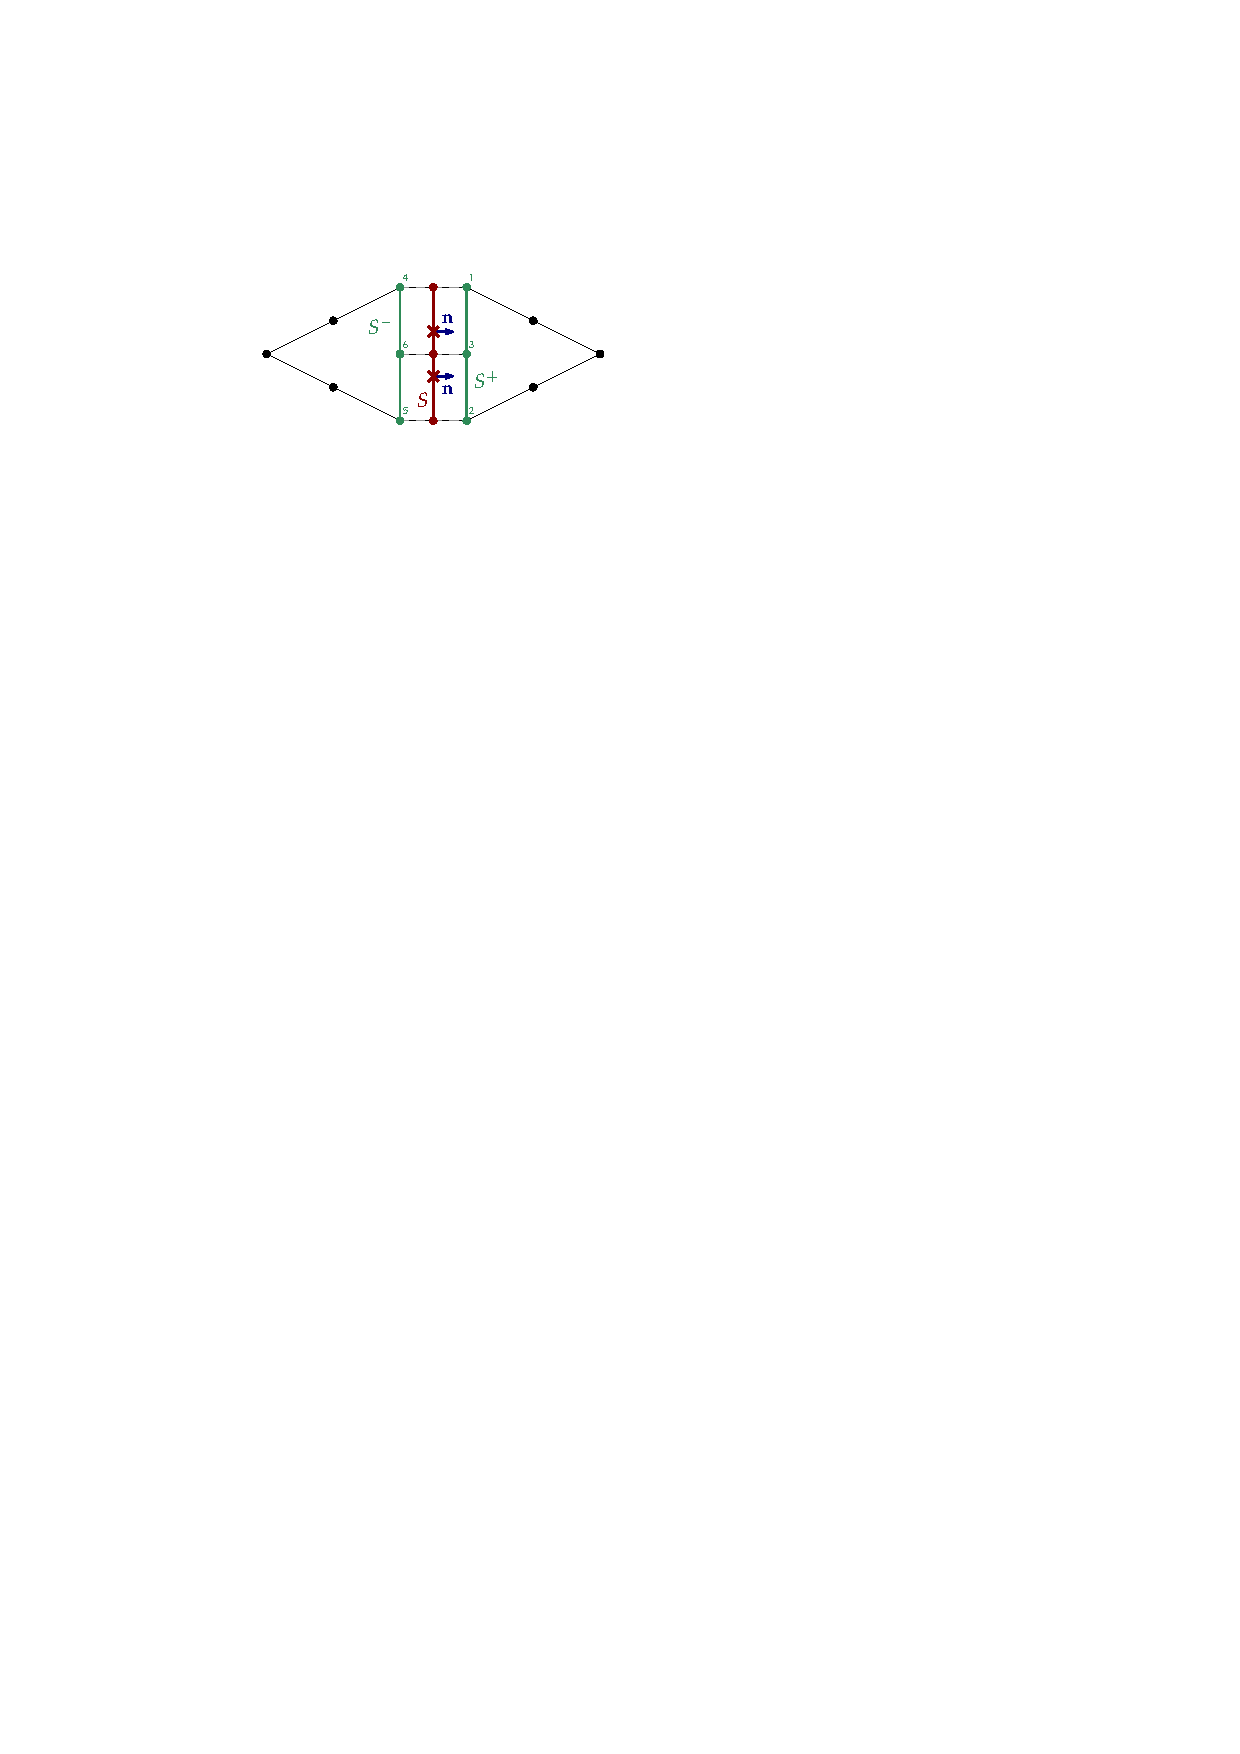
\includegraphics[width=.6\textwidth]{figures/cohesive2d}
  \caption{Cohesive element in 2D for quadratic triangular elements
    T6.}
  \label{fig:smm:coh:cohesive2d}
\end{figure}

\begin{figure}
  \centering
  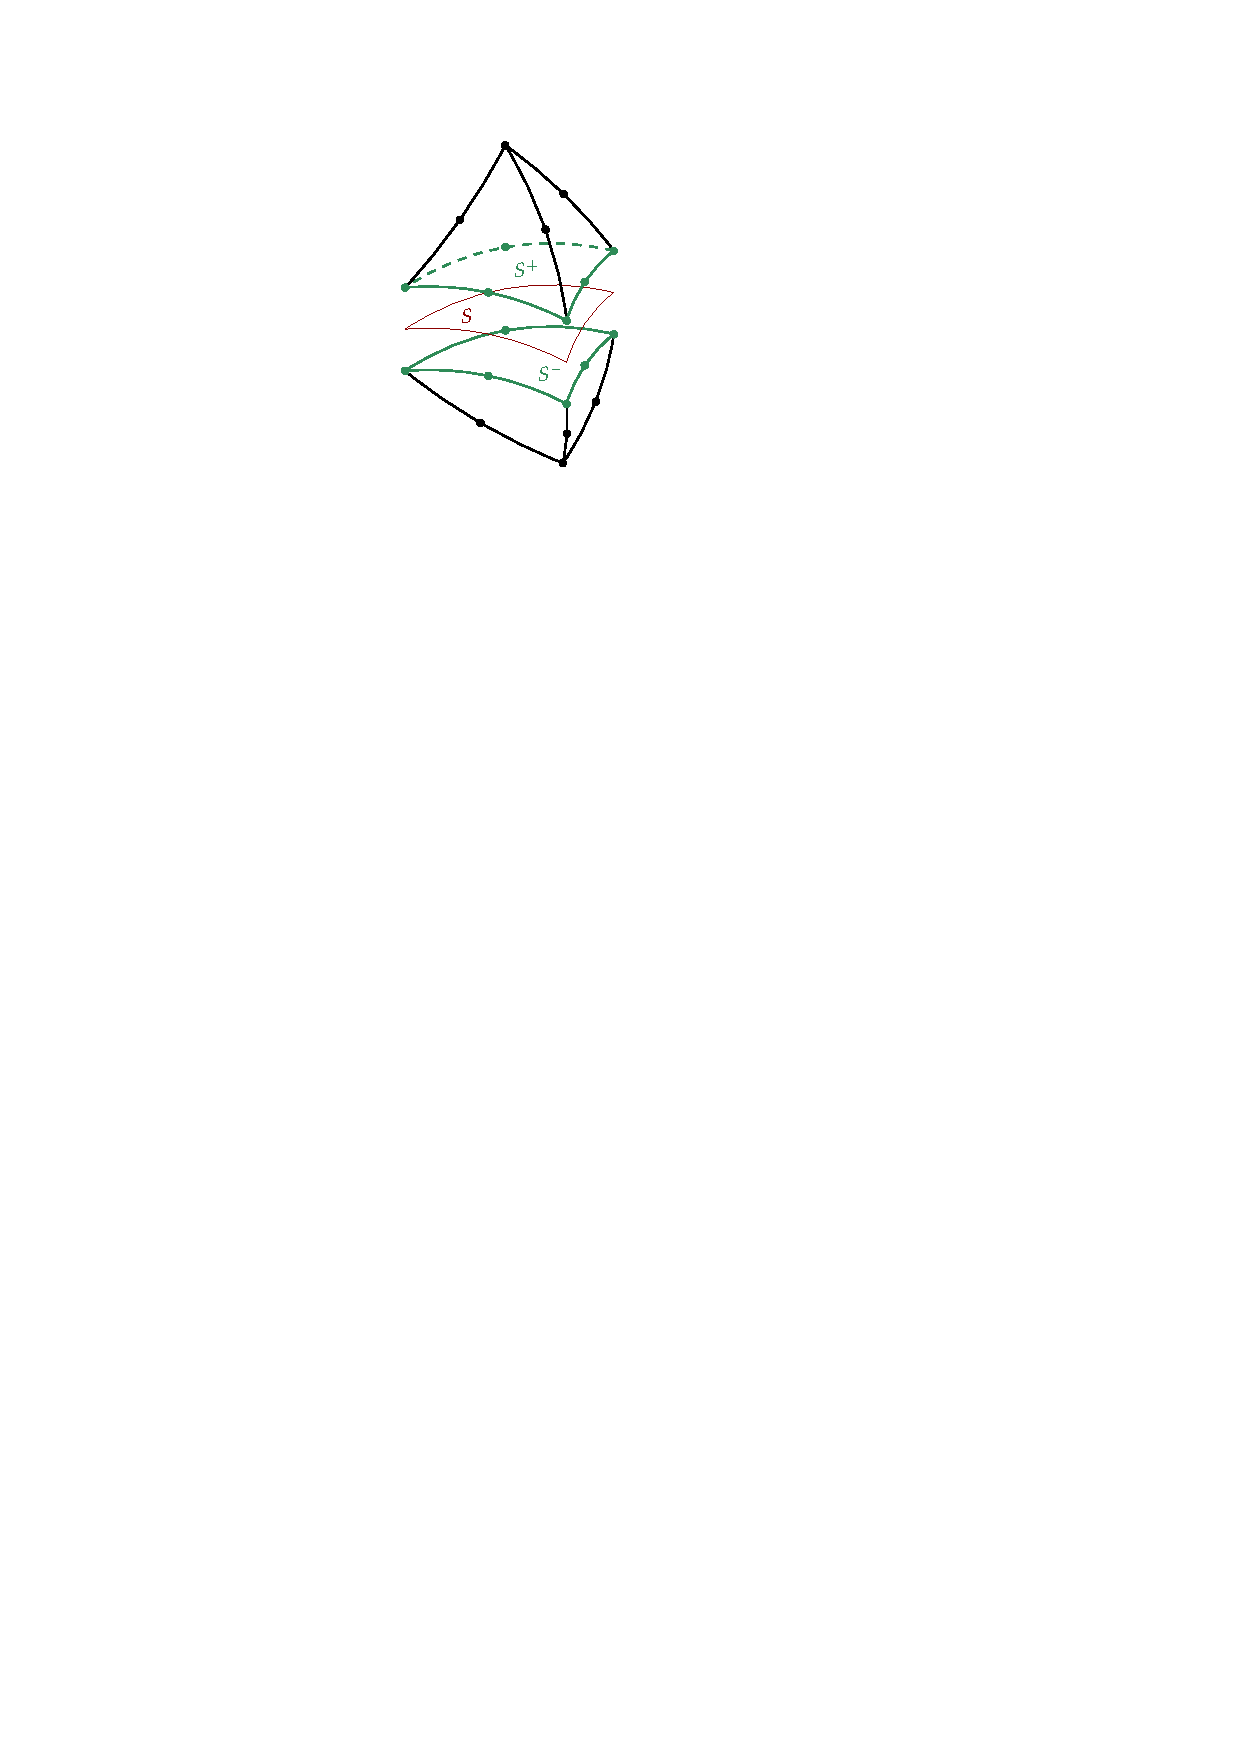
\includegraphics[width=.25\textwidth]{figures/cohesive3d}
  \caption{Cohesive element in 3D for quadratic tetrahedrons T10.}
  \label{fig:smm:coh:cohesive3d}
\end{figure}

Cohesive elements consist of a couple of surface elements which are
coincident in space when the opening displacement is zero. Two
schematics of cohesive elements in 2D and 3D can be seen in
Figures~\ref{fig:smm:coh:cohesive2d}
and~\ref{fig:smm:coh:cohesive3d}. The two surface elements, denoted by
$S^-$ and $S^+$, must be of the same type and they correspond to the
facet element of the standard elements. All the computations are done
on the middle surface $S$, whose nodal coordinates are just the
average between those of $S^+$ and $S^-$.

In order to track normal and tangential openings, it is convenient to
define a unique normal direction $\vec{n}$ for each quadrature point
of the cohesive element. By convention the normal points from $S^-$ to
$S^+$. The opening displacement vector is:
\begin{equation}
  \label{eq:opening_displacement}
  \vec{\Delta} (\vec{s}) = \sum_{n=1}^N \llbracket \vec{x}_n \rrbracket N_n (\vec s)
\end{equation}
where $N_n$ are the shape functions of the cohesive element (they are
exactly the same of those of a single surface element) and
\begin{equation}
  \label{eq:disp_difference}
  \llbracket \vec{x}_n \rrbracket = \vec{x}_n^+ - \vec{x}_n^-
\end{equation}
in which $\vec{x}_n^\pm$ for $n=1,\dots,N$ are the current coordinates
of the nodes.

The quantities that have been defined so far are sufficient to
completely define the cohesive traction per unit deformed
area. As the tangential direction $\vec{t}$ depends on the normal one
$\vec{n}$, equation~\eqref{eq:smm:coh:tractions} can be rewritten as:
\begin{equation}
  \vec{T} = \left[ \frac{\beta^2}{\kappa} \vec{\Delta} +
    \left( 1- \frac{\beta^2}{\kappa}\right)
    \left( \vec{\Delta} \cdot \vec{n}\right) \vec{n} \right]
  \frac{\sigma_\mathrm{c}}{\delta}
  \left( 1- \frac{\delta}{\delta_\mathrm{c}} \right) =
  \vec{T}(\vec{\Delta}, \vec{n})
\end{equation}
 By interpolation it is now possible to derive the nodal
forces as:
\begin{equation}
  f_{in}^\pm = \mp \int_{S_0} T_i N_n\, \mathrm{d}S_0
\end{equation}
in which the integral extends over the undeformed middle surface $S_0$
of the cohesive element.

\begin{figure}
  \centering
  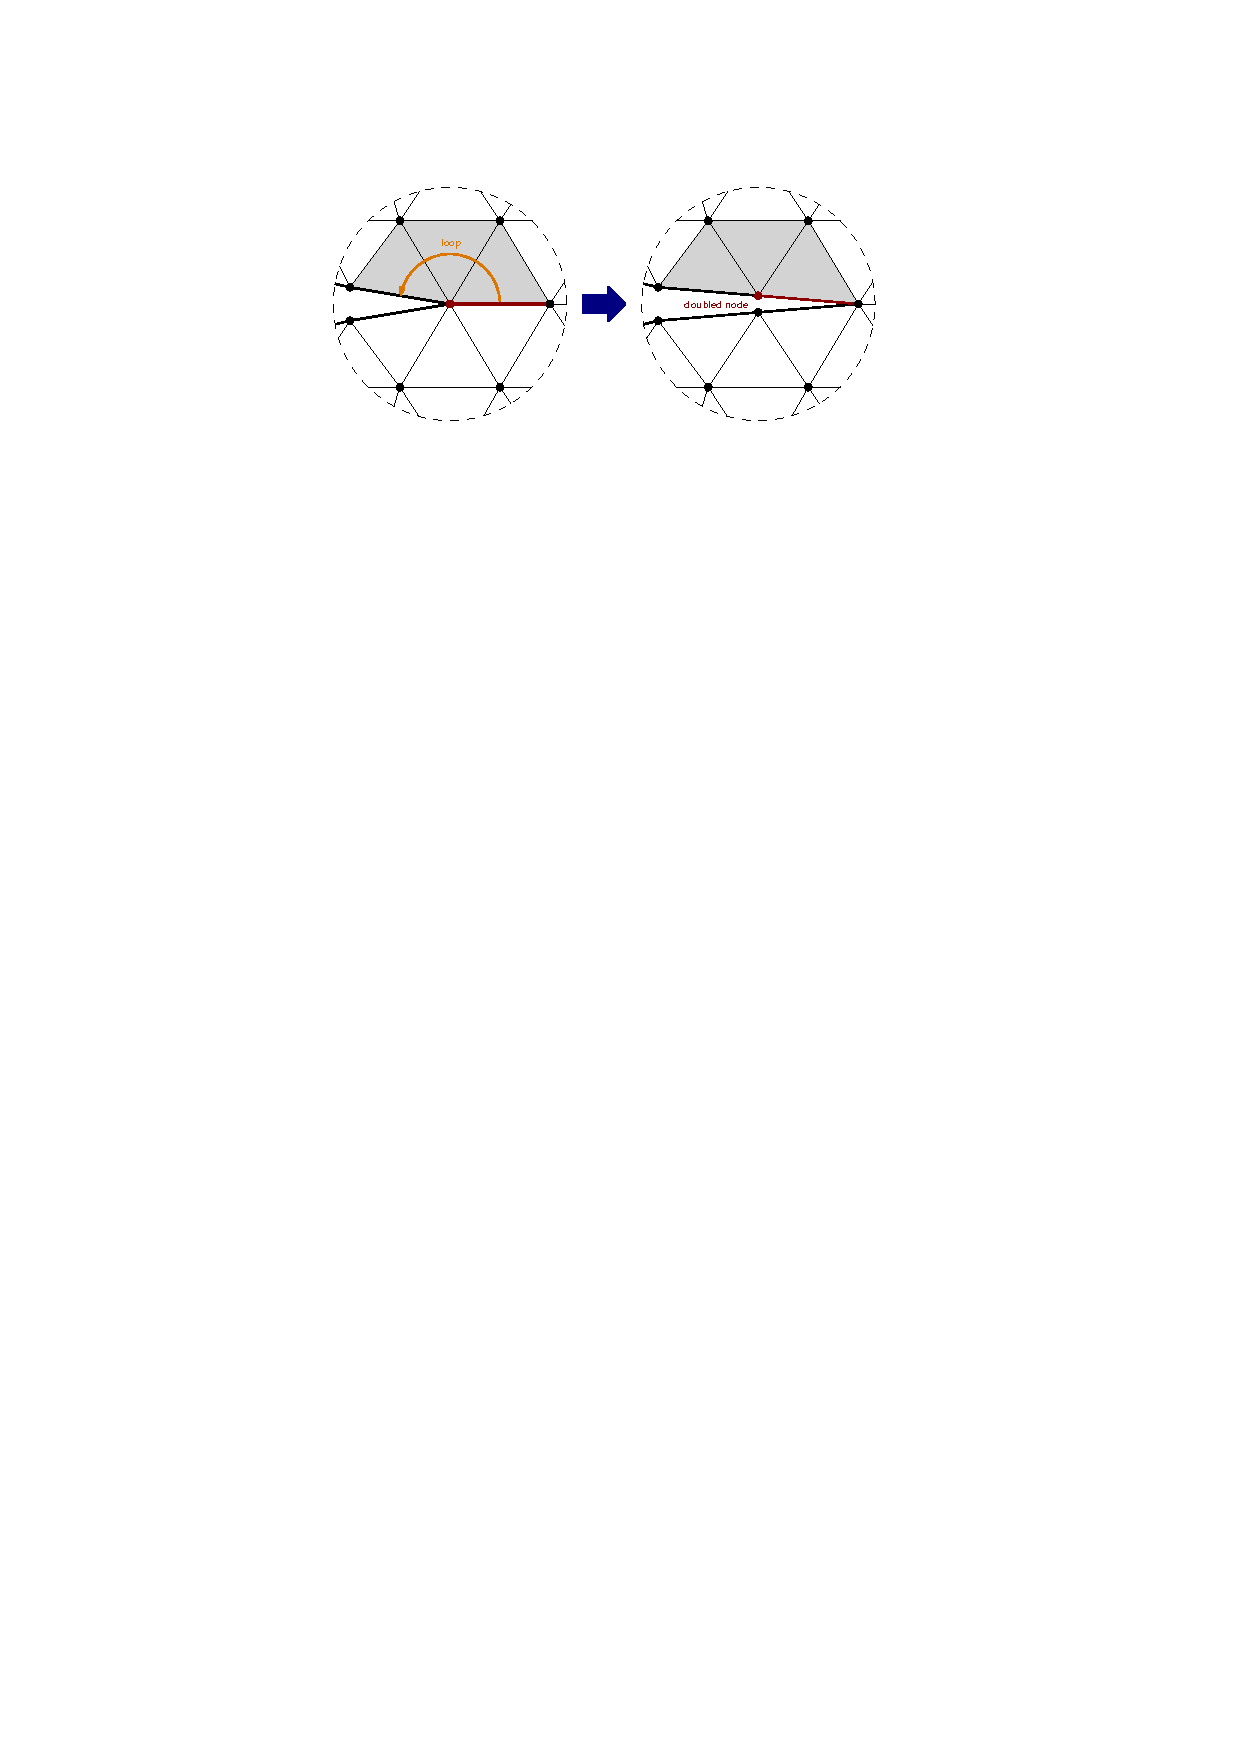
\includegraphics[width=.9\textwidth]{figures/insertion}
  \caption{Insertion of a cohesive element.}
  \label{fig:smm:coh:insertion}
\end{figure}

Cohesive element insertion can be either realized at the beginning of
the simulation or it can be carried out dynamically during the
simulation. The first approach is called \emph{intrinsic}, the
second one \emph{extrinsic}. When an element is present from the
beginning, a bilinear or exponential cohesive law should be used
instead of a linear one. A bilinear law works exactly like a linear
one except for an additional parameter $\delta_0$ separating an
initial linear elastic part from the linear irreversible one. The
exponential law will be described later in the manual.

In dynamic cohesive element insertion, normal and tangential stresses
along the edges of standard elements are used to compute the effective
stress
\begin{equation}
  \sigma_\mathrm{eff} = \sqrt{\sigma_\mathrm{n}^2 +
    \frac{\tau_\mathrm{nt}^2}{\beta^2}}
\end{equation}
where the indices $n$ and $t$ respectively refer to normal and
tangential directions. Obviously, if $\sigma_\mathrm{n}$ is
compressive, its contribution is not considered. The computed
effective stress $\sigma_\mathrm{eff}$ is monitored, and when it
overcomes a threshold stress on a certain edge, a new cohesive element
is inserted. New nodes are added and the element connectivity is
updated (see Figure~\ref{fig:smm:coh:insertion}). This topological
mesh changing technique is very convenient because it allows
simulating crack propagation without remeshing the domain.

\begin{table}[!htb]
\begin{center}
\begin{tabular}{l|llcc}
\toprule
Element type & Facet type & Order & \# nodes & \# quad. points  \\
\midrule
\texttt{\_cohesive\_1d\_2} & \texttt{\_point\_1} & linear & 2 & 1  \\
\hline
\texttt{\_cohesive\_2d\_4} & \texttt{\_segment\_2} & linear & 4 & 1  \\
\texttt{\_cohesive\_2d\_6} & \texttt{\_segment\_3} & quadratic & 6 & 2  \\
\hline
\texttt{\_cohesive\_3d\_6} & \texttt{\_triangle\_3} & linear & 6 & 1  \\
\texttt{\_cohesive\_3d\_12} & \texttt{\_triangle\_6} & quadratic & 12 & 3  \\
\bottomrule
\end{tabular}
\end{center}
\caption{Some basic properties of the cohesive elements in \akantu.}
\label{tab:cohesive_elements}
\end{table}

For the static analysis of the structures containing cohesive
elements, the stiffness of the cohesive elements should also be added
to the total stiffness of the structure. Considering a typical
cohesive element as explained in Figure~\ref{fig:smm:coh:cohesive2d},
the opening displacement along the mid-surface can be written as:

\begin{equation}
  \label{eq:opening}
  \delta(\xi) = [[\mat{u}]] \mat{N}(\xi) =
  \begin{bmatrix}
    u_3-u_0 & u_4-u_1 & u_5-u_2\\
    v_3-v_0 & v_4-v_1 & v_5-v_2
  \end{bmatrix}
  \begin{bmatrix}
    N_0(\xi) \\ N_1(\xi) \\ N_2(\xi)
  \end{bmatrix} =
  \mat{N A U}
\end{equation}

The \mat{U} , \mat{A} and \mat{N} are as following:

\begin{equation}
  \mat{U} = \left [
    \begin{array}{c c c c c c c c c c c c}
      u_0 & v_0 & u_1 & v_1 & u_2 & v_2 & u_3 & v_3 & u_4 & v_4 & u_5 & v_5
    \end{array}\right ]
\end{equation}


\begin{equation}
  \mat{A} = \left [\begin{array}{c c c c c c c c c c c c}
      1 & 0 & 0 & 0& 0 & 0 & -1& 0 & 0 &0 &0 &0\\
      0 &1& 0&0 &0 &0 &0 & -1& 0& 0 & 0 &0\\
      0 &0& 1&0 &0 &0 &0 & 0& -1& 0 & 0 &0\\
      0 &0& 0&1 &0 &0 &0 & 0& 0& -1 & 0 &0\\
      0 &0& 0&0 &1 &0 &0 & 0& 0& 0 & -1 &0\\
      0 &0& 0&0 &0 &1 &0 & 0& 0& 0 & 0 &-1
    \end{array} \right ]
\end{equation}


\begin{equation}
  \mat{N} = \begin{bmatrix}
    N_0(\xi) & 0 & N_1(\xi) &0 & N_2(\xi) & 0\\
    0 & N_0(\xi)& 0 &N_1(\xi)& 0 & N_2(\xi)
  \end{bmatrix}
\end{equation}

The consistent stiffness matrix for the element is obtained as

\begin{equation}
  \label{eq:cohesive_stiffness}
  \mat{K}    =    \delta    \mat{U}^T    \int_{\Gamma_c}    {\mat{P}^t
    \frac{\partial{\mat{t}}} {\partial{\delta}} \mat{P} d
    \Gamma \Delta \mat{U}}
\end{equation}

In which the tangent matrix is calculated based on the equation \ref
{eq:tangent_cohesive} after performing necessary derivation:

\begin{equation}
  \label{eq:tangent_cohesive}
  \frac{\partial{\mat{t}}} {\partial{\delta}} = \hat{\mat{t}} \otimes
  \frac                       {\partial{(t/\delta)}}{\partial{\delta}}
  \frac{\hat{\mat{t}}}{\delta}+ \frac{t}{\delta}  [ \beta^2 \mat{I} +
  (1-\beta^2) (\mat{n} \otimes \mat{n})]
\end{equation}



%%% Local Variables:
%%% mode: latex
%%% TeX-master: "manual"
%%% End:
